%!TeX program = xelatex
\documentclass[12pt,hyperref,a4paper,UTF8]{ctexart}
\usepackage{zjureport}
\usepackage{tikz}
\usepackage{pgfplots}
\definecolor{cmdbg}{rgb}{0.92,0.92,0.92}

%%-------------------------------正文开始---------------------------%%
\begin{document}

%%-----------------------封面--------------------%%
\cover


\thispagestyle{empty} % 首页不显示页码

%%--------------------------目录页------------------------%%
\newpage
\tableofcontents

%%------------------------正文页从这里开始-------------------%
\newpage

\section{实验分工}

\begin{table}[!htbp]
    \centering
    \begin{tabular}{c|c}
        \hline
        姓名 & 分工 \\
        \hline
        刘韬 & lab1(包括bonus),lab2,lab3,系统功能调试,小组报告撰写 \\
        周龙 & lab4,lab5,lab6 \\
        \hline
    \end{tabular}
    \caption{实验分工}
    \label{table1}
\end{table}

\section{实验概述}
% 本模板主要适用于一些课程的平时论文以及期末论文,默认页边距为2.5cm,中文宋体,英文Times New Roman,字号为12pt(小四)。
\subsection{实验目的}
\begin{enumerate}
    \item 设计并实现一个精简型单用户SQL引擎MiniSQL,允许用户通过字符界面输入SQL语句实现基本的增删改查操作,并能够通过索引来优化性能。
    \item 通过对MiniSQL的设计与实现,提高学生的系统编程能力,加深对数据库管理系统底层设计的理解。
\end{enumerate}

\subsection{实验需求}
\begin{enumerate}
    \item 数据类型:要求支持三种基本数据类型:\verb|integer,char(n),float|。
    \item 表定义:一个表可以定义多达32个属性,各属性可以指定是否为unique,支持单属性的主键定义。
    \item 索引定义:对于表的主属性自动建立B+树索引,对于声明为unique的属性也需要建立B+树索引。
    \item 数据操作: 可以通过and或or连接的多个条件进行查询,支持等值查询和区间查询。支持每次一条记录的插入操作;支持每次一条或多条记录的删除操作。
    \item 使用源代码管理工具(如Git)进行代码管理,代码提交历史和每次提交的信息清晰明确;同时编写的代码应符合代码规范,具有良好的代码风格。
\end{enumerate}

\paragraph{需要支持的SQL语句} 实验应当支持以下SQL语句:
\begin{minted}
    [
        linenos,
        breaklines,
        bgcolor = cmdbg,
        fontsize=\footnotesize,
        frame=lines
    ]{SQL}
create database db0;
drop database db0;
show databases;
use db0;
show tables;
create table t1(a int, b char(20) unique, c float, primary key(a, c));
create table t1(a int, b char(0) unique, c float, primary key(a, c));
create table t1(a int, b char(-5) unique, c float, primary key(a, c));
create table t1(a int, b char(3.69) unique, c float, primary key(a, c));
create table t1(a int, b char(-0.69) unique, c float, primary key(a, c));
create table student(
  sno char(8),
  sage int,
  sab float unique,
  primary key (sno, sab)
);
drop table t1;
create index idx1 on t1(a, b);
-- "btree" can be replaced with other index types
create index idx1 on t1(a, b) using btree;
drop index idx1;
show indexes;
select * from t1;
select id, name from t1;
select * from t1 where id = 1;
-- note: use left association
select * from t1 where id = 1 and name = "str";
select * from t1 where id = 1 and name = "str" or age is null and bb not null;
insert into t1 values(1, "aaa", null, 2.33);
delete from t1;
delete from t1 where id = 1 and amount = 2.33;
update t1 set c = 3;
update t1 set a = 1, b = "ccc" where b = 2.33;
quit;
execfile "a.txt";
\end{minted}

\subsection{实验环境}

\begin{itemize}
    \item 基于WSL2--ubuntu进行开发,通过vscode连接至Linux子系统.
    \item 基于MacOS进行开发,使用clang编译.
\end{itemize}

\section{系统架构和模块概述}

\subsection{系统架构}

最终我们向用户呈现的是一个命令行界面,用户可以通过命令行输入SQL语句,MiniSQL会解析这些SQL语句并执行相应的操作。MiniSQL的整体架构如下图所示:

\begin{figure}[!htbp]
    \centering
    \includegraphics[width=0.8\textwidth]{figures/structure.png}
    \caption{MiniSQL系统架构}
    \label{fig1}
\end{figure}

系统接收到SQL语句后,通过SQL Parser生成语法树,然后通过executor(由Planner and Executor调用下层模块生成)调用Catalog Manager、Record Manager和Index Manager等模块来执行相应的操作。
Catalog Manager负责表的元数据管理,Record Manager负责表的记录管理,Index Manager负责索引的管理。而这三个模块都是基于Buffer Manager提供的缓冲区管理服务。
Buffer Manager负责缓冲区的管理,调用Disk Manager来读写文件。

每个DB Storage Engine Instance对应了一个数据库实例(即通过CREATE DATABSAE创建的数据库)。
在每个数据库实例中,用户可以定义若干表和索引,表和索引的信息通过Catalog Manager、Index Manager和Record Manager进行维护。
我们实现的系统支持使用多个数据库实例,不同的数据库实例可以通过USE语句切换(即类似于MySQL的切换数据库)。

\subsection{模块概述}

系统架构是自上而下的叙述系统的工作原理和工作流程,在具体实现时应当是自下而上进行模块支持。下面我们将对系统的各个模块进行介绍。详细的实现报告请参考个人报告。

\subsubsection{DiskManager}

DiskManager是系统最底层的模块,负责与磁盘进行交互,负责DB File中数据页的分配和回收,以及数据页中数据的读取和写入。在我们的实现中
为了管理数据库中的文件,我们需要实现一个对磁盘进行读写的类 DiskManager,它的功能是对数据中的page(基本数据单元)进行allocation和 de allocation,执行从磁盘中进行读写page的操作。
除了存储数据的数据页,我们还需要一些元数据来帮助和加速数据页的管理,于是位图页就自然的出现了。
我们将一个位图页和它所管理的一段连续的数据页称作数据库文件中的一个分区(extent)。为了提高存储的容量,我们使用一个额外的元信息页来存储各个分区的信息。
这种套娃的方式可以使磁盘文件能够维护更多的数据页信息。DiskManager所实现的数据结构如图\ref{fig2}所示,其中包括了数据页、位图页和元信息页。

\begin{figure}[!h]
    \centering
    \includegraphics[width=0.8\textwidth]{figures/disk_data.png}
    \caption{DiskManager模块}
    \label{fig2}
\end{figure}

数据页就是存储数据的基本单位,位图页用于管理数据页的分配和回收,元信息页用于存储各个分区的信息。以下是位图页的设计:

\begin{figure}[!h]
    \centering
    \includegraphics[width=0.8\textwidth]{figures/Bitmap_page.png}
    \caption{位图页设计}
    \label{fig:bitmap}
\end{figure}

\paragraph{bitmap page}
位图页的大小与数据页的大小一致,如\ref{fig:bitmap}所示,
位图页由Bitmap Page Meta 和 Bitmap Content 两部分组成。
Bitmap Page Meta就是位图页的元数据,含当前已经分配的页的数量(page\_allocated\_)以及下一个空闲的数据页(next\_free\_page\_)。
Bitmap Content使用char数组来记录数据,其容量大小是 MAX\_CHARS = PageSize - 2 * sizeof(uint32\_t),
每个bit的含义是对应的页是否被分配,一个char的大小是8bits,位图页对外提供分配、回收数据页和判断数据页是否可用的接口,内部实现是对上述数组的管理。

DiskManager具有向磁盘读写物理页,分配和回收页的功能。为了更好地管理数据,我们在前面设置了元数据页,但对于上层的程序而言,数据管理器提供的应当是连续的数据页,即逻辑页号。因此我们需要在这里对逻辑页和物理页进行映射,使得上层能够无感知地获得数据页。映射示意图\ref{fig:phy-log}

\begin{figure}[!ht]
    \centering
    \includegraphics[width=0.8\textwidth]{figures/phy-log.png}
    \caption{逻辑页和物理页映射}
    \label{fig:phy-log}
\end{figure}

\subsubsection{BufferPoolManager}

Buffer Manager 负责缓冲区的管理,主要功能包括:
\begin{itemize}
    \item 根据需要,从磁盘中读取指定的数据页到缓冲区中或将缓冲区中的数据页转储(Flush)到磁盘
    \item 实现缓冲区的替换算法,当缓冲区满时选择合适的数据页进行替换;
    \item 记录缓冲区中各页的状态,如是否是脏页(Dirty Page)、是否被锁定(Pin)等;
    \item 提供缓冲区页的锁定功能,被锁定的页将不允许替换。
\end{itemize}

为提高磁盘 I/O 操作的效率,缓冲区与文件系统交互的单位是数据页(Page),数据页的大小应为文件系统与磁盘交互单位的整数倍。在本实验中,数据页的大小默认为 4KB。

对于上述要实现的功能,我们首先需要实现缓冲区的替换算法,本实验中我们实现了LRU算法和CLOCK算法。LRU算法是一种最近最少使用算法,即当缓冲区满时,选择最近最少使用的页进行替换。CLOCK算法是一种近似LRU算法,它维护一个指针,指向最近访问的页,当缓冲区满时,选择指针指向的页进行替换。

然后我们实现了缓冲区的管理,即实现了缓冲区的初始化、读取数据页、写入数据页、将数据页标记为脏页、将数据页标记为锁定页等功能。缓冲池管理器为上层提供读取数据的接口,上层只要输入page\_id,即可获得数据页的内容。对内调用DiskManager,将数据页读取到缓冲区中。实现了良好的封装,上层无需关心数据页的具体存储位置,只需关心逻辑页号。

在后续的开发中,涉及到页面的操作都只需要通过BufferPoolManager类来完成。

\subsubsection{Record Manager}

\paragraph{Record design}
我们的记录包含以下几个概念:

\begin{itemize}
    \item \textbf{Column}:用于定义和表示数据表中的某一个字段,即包含了这个字段的字段名、字段类型、是否唯一等等;
    \item \textbf{Schema}:用于表示一个数据表或是一个索引的结构。一个Schema由一个或多个的Column构成;
    \item \textbf{Field}:它对应于一条记录中某一个字段的数据信息,如存储数据的数据类型,是否是空,存储数据的值等等;
    \item \textbf{Row}: 用于表示一条记录,即一行数据,由多个Field组成;
\end{itemize}

这是我们数据在数据库中的组织方式,但是为了将其持久化地存储在硬盘中,我们需要使用序列化和反序列化地方法,将其转化为字节流。

Record Manager 负责管理数据表中记录。所有的记录以堆表(Table Heap)的形式进行组织。Record Manager 的主要功能包括:记录的插入、删除与查找操作,并对外提供相应的接口。其中查找操作返回的是符合条件记录的起始迭代器,对迭代器的迭代访问操作由执行器(Executor)进行。

\paragraph{Table Heap}

堆表是由多个数据页构成的链表,每个数据页中包含一条或多条记录,支持非定长记录的存储。不要求支持单条记录的跨页存储(即保证所有插入的记录都小于数据页的大小)。堆表中所有的记录都是无序存储的。每条记录都有一个独特的\verb|RowId|标记其所在的位置。
利用这个\verb|RowId|,我们可以在堆表中快速定位到一条记录。table heap的结构如下:

堆表中的每个数据页都由表头(Table Page Header)、空闲空间(Free Space)和已经插入的数据(Inserted Tuples)三部分组成,
表头在页中从左往右扩展,记录了PrevPageId、NextPageId、FreeSpacePointer以及每条记录在TablePage中的偏移和长度;
插入的记录在页中从右向左扩展,每次插入记录时会将FreeSpacePointer的位置向左移动。

\begin{figure}[!ht]
    \centering
    \includegraphics[width=0.8\textwidth]{figures/table_heap.png}
    \caption{Table Page结构}
    \label{fig:table_page}
\end{figure}

\subsubsection{Index Manager}

Index Manager 负责索引的管理,主要功能包括:包括:索引(B+树等形式)的创建和删除,索引键的等值查找,索引键的范围查找(返回对应的迭代器),以及插入和删除键值等操作,并对外提供相应的接口。

为了提高搜索的效率,我们实现基于磁盘的B+树动态索引结构。首先完成b+树数据结构的实现,然后建立在此基础上建立索引。
B+树索引中的节点大小应与缓冲区的数据页大小相同,B+树的叉数由节点大小与索引键大小计算得到。

我们定义了\verb|IndexRootsPage|来存储所有Index的b+树的根节点的信息,主要包括index\_id, root\_page\_id等等,用于在系统启动时加载所有的索引。

为了给executor提供使用接口,我们实现了迭代器用于索引的查找操作。
在后续的开发中,我们只需要通过BPlusTree类的Begin和End方法来获取迭代器,然后通过迭代器来遍历B+树中的键值对。

\subsubsection{Catalog Manager}

\paragraph{Catalog Meta}
catalog是用来管理表和索引的数据信息的。表和索引的数据以tableInfo和indexInfo的类存储,这个类中包含表和索引的元信息metadata以及一些需要反序列化存储的信息。每张表和索引将存储在一张单独的page中,这个page存储的是对应表或索引序列化后的数据。而为了记录每张表和索引储存在那张page上,还需要一张总page来记录每张表和索引与各自page的对应关系,这张总page上的数据即为catalogMeta,
其信息以序列化的形式储存在数据库的CATALOG\_META\_PAGE\_ID数据页中,CATALOG\_META\_PAGE\_ID的值为零。

\paragraph{Catalog Manager}

catalogManager用来管理目录元信息和数据页中表和索引的信息。当其初始化时,会加载元数据,把tableInfo和indexInfo放在内存中等待使用。通过catalogManager类里的方法可以对表与索引进行操作,包括创建、删除等。这些方法可以由上层模块调用,获取表与索引中的信息。

catalogManager可以调用buffer pool manager的方法,获取与存储各种元数据;同时会被executor调用,进行表与索引的增删。

\subsubsection{Planner and Executor}

这个模块负责执行输入的sql语句。首先解释器parser用输入的SQL语句生成语法树,然后简单的语法树可以直接处理,复杂的语法树例如插入、删除等交由planner生成计划树,将一系列计划交给executor执行。

\paragraph{Planner}
Planner(执行计划生成器)的主要功能是根据解释器(Parser)生成的语法树,通过Catalog Manager 提供的信息检查语法树中的信息是否正确,如表、列是否存在,谓词的值类型是否与column类型对应等等,随后将这些词语转换成可以理解的各种 c++ 类。解析完成后,Planner根据改写语法树后生成的Statement结构,生成对应的Plannode,并将Plannode交由Executor进行执行。
\paragraph{Executor}
Executor(执行器)的主要功能是遍历Planner生成的计划树,将树上的 PlanNode 替换成对应的 Executor,并调用 Record Manager、Index Manager 和 Catalog Manager 提供的相应接口进行执行。Executor采用的是火山模型,提供迭代器接口,每次调用时会返回一个元组和相应的 RID,直到执行完成。
本实验中executor模块采用的算子执行模型为火山模型,即iterator model。每个算子有两个方法:init和next,init进行初始化,next向下层算子请求下一条数据。next的返回类型为bool,当返回false时说明没有下一条数据,执行结束。

\subsubsection{SQL Parser}
程序流程控制,即“启动并初始化 → ‘接收命令、处理命令、显示命令结果’循环 → 退出”流程。
接收并解释用户输入的命令,生成命令的内部数据结构表示,同时检查命令的语法正确性和部分语义正确性,对正确的命令生成语法树,然后调用执行器层提供的函数执行并显示执行结果,对不正确的命令显示错误信息。

\subsubsection{Recovery Manager}
Recovery Manager 负责管理和维护数据恢复的过程,实现一个纯内存的数据恢复模块即可,包括:
\begin{itemize}
    \item 日志结构的定义
    \item 检查点CheckPoint的定义
    \item 执行Redo、Undo等操作,处理插入、删除、更新,事务的开始、提交、回滚等日志,将数据库恢复到宕机之前的状态
\end{itemize}

日志在内存中以LogRec的形式表现.本实验不考虑日志的落盘,用一个unordered\_map简易的模拟一个KV Database,并直接在内存中定义一个能够用于插入、删除、更新,事务的开始、提交、回滚的日志结构。那么数据的恢复就很简单,redo的事务可以直接对内存进行插删等操作来进行即可。

\paragraph{思考题}
本模块中,为了简化实验难度,我们将Recovery Manager模块独立出来。如果不独立出来,真正做到数据库在任何时候断电都能恢复,同时支持事务的回滚,Recovery Manager应该怎样设计呢?此外,CheckPoint机制应该怎样设计呢?

\begin{itemize}
    \item 首先是LogRec的结构,不再是target\_key和target\_val,应该包含table\_name,index\_name,rid,column等,LogRecType也应该更加细化,例如kDelete要细分为kDeleteFromTable,kDeleteRow。
    \item Redo,Undo,Rollback时,不能直接修改,而是调用Catalog Manager以及table\_heap的函数来实现,比如删除某一条数据时:(如果是回滚事务,需要调用table\_heap中的RollbackDelete()函数)
\end{itemize}

\begin{minted}
    [
        linenos,
        breaklines,
        bgcolor = cmdbg,
        fontsize=\footnotesize,
        frame=lines
    ]{cpp}
    TableInfo *table_info;
    dbs_[current_db_]->catalog_mgr_->GetTable(log_rec.table_name,table_info);
    table_info->GetTableHeap()->MarkDelete(log_rec.rid,log_rec.txn);
\end{minted}
\begin{itemize}
    \item 创建日志的函数要根据LogRec结构的修改做出对应的修改,在执行器执行语句时需要调用这些函数创建日志。
    \item 要专门有一张Page记录日志,当发生crash后需要将日志Load上来。参考table和index的记录方式,可以对日志进行序列化和反序列化操作。
    \item 采用Fuzzy Checkpoint,Innodb每次取最老的modified page(last checkpoint)对应的LSN,再将此脏页的LSN作为Checkpoint点记录到日志文件,意思就是“此LSN之前的LSN对应的日志和数据都已经flush到redo log。当mysql crash的时候,Innodb扫描redo log,从last checkpoint开始apply redo log到buffer pool,直到last checkpoint对应的LSN等于Log flushed up to对应的LSN,则恢复完成。
\end{itemize}

\section{测试样例和功能测试}

\subsection{测试样例}

我们修改的测试用例包括,详尽的修改见个人报告:
\begin{itemize}
    \item lab1:CLOCKReplacerTest
    \item lab2:TableHeapTest
    \item lab3: BPlusTreeTest
\end{itemize}

下面是测试的结果:

\begin{figure}[!ht]
    \centering
    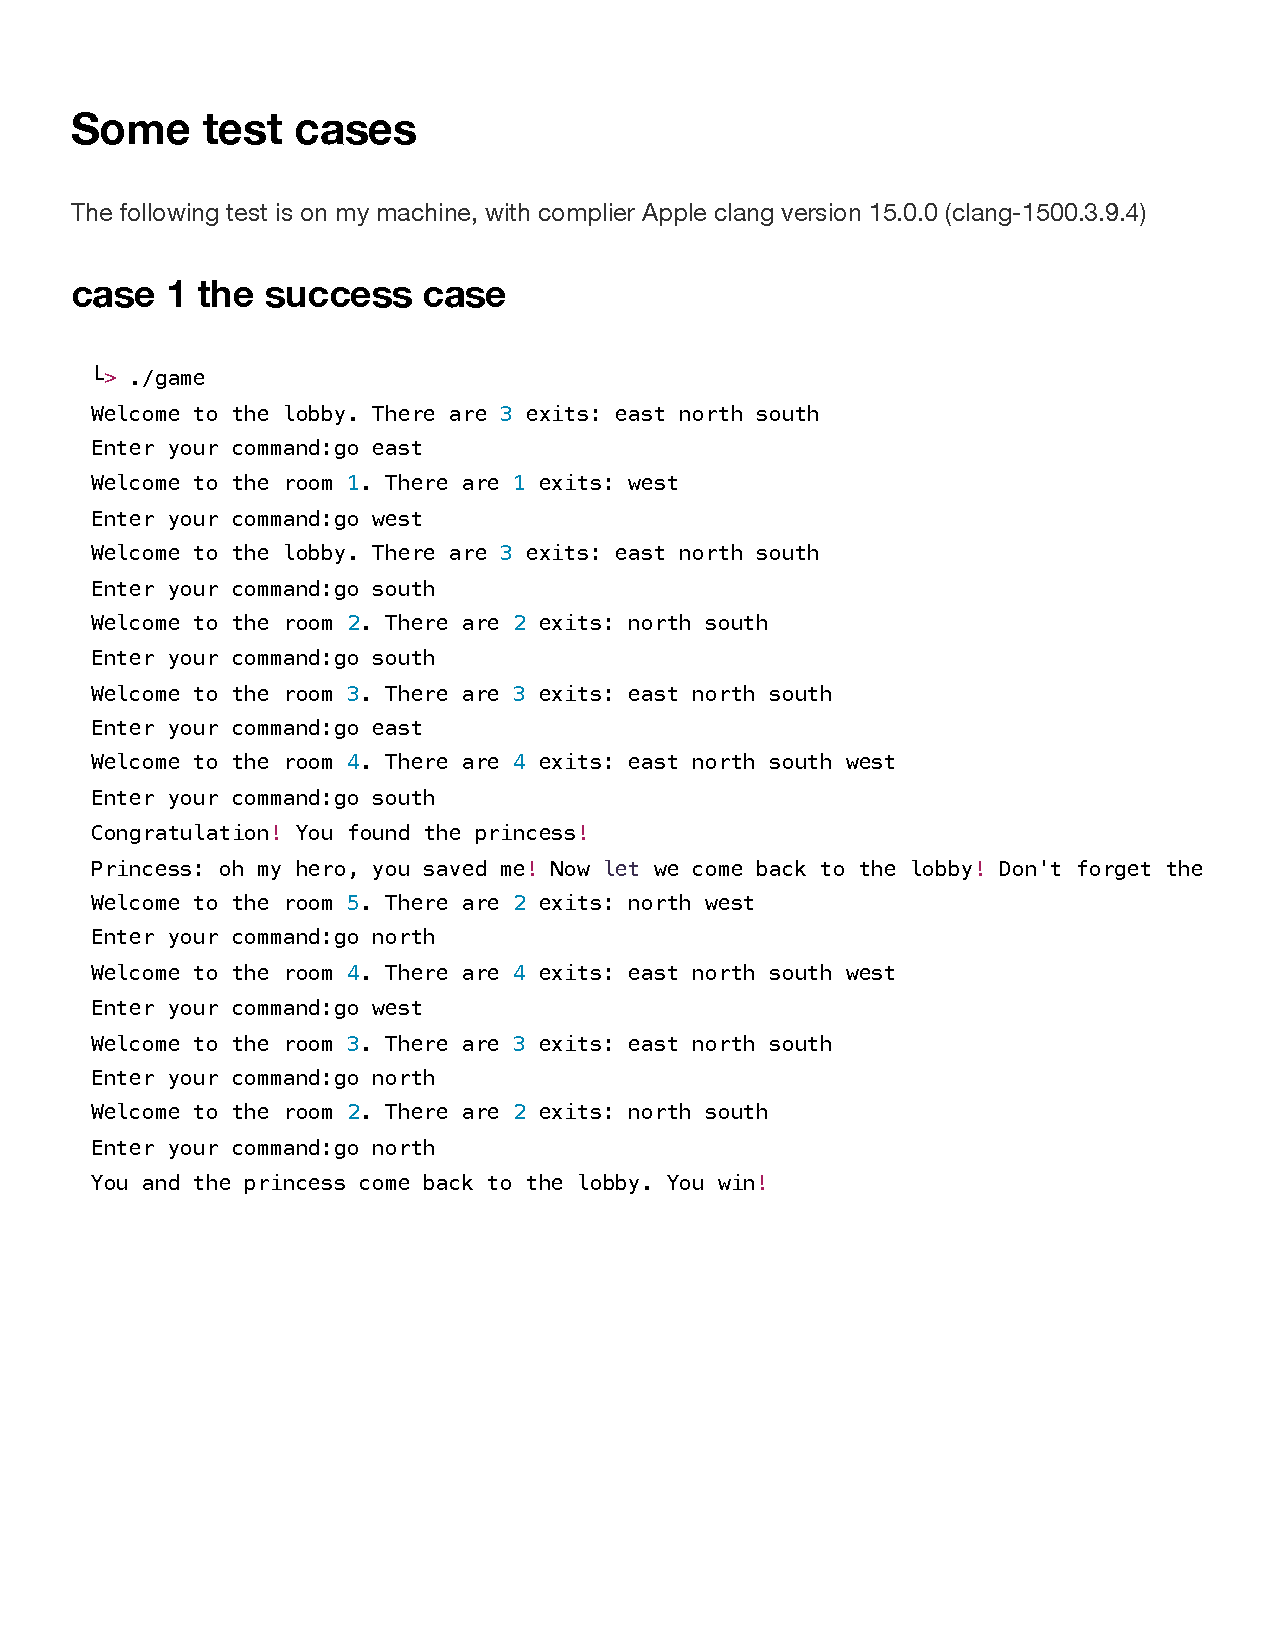
\includegraphics[width=0.8\textwidth]{figures/test.png}
    \caption{测试结果}
    \label{fig:test1}
\end{figure}

全部的样例测试都通过。

\subsection{功能测试}

我们对MiniSQL进行了功能测试,测试了MiniSQL的各个功能,包括:
\begin{minted}
    [
        linenos,
        breaklines,
        bgcolor = cmdbg,
        fontsize=\footnotesize,
        frame=lines
    ]{SQL}
create database db0;
use db0;
create table account(
    id int, 
    name char(16) unique, 
    balance float, 
    primary key(id)
);

execfile "../sql_gen/account00.txt";
execfile "../sql_gen/account01.txt";
execfile "../sql_gen/account02.txt";
execfile "../sql_gen/account03.txt";
execfile "../sql_gen/account04.txt";
execfile "../sql_gen/account05.txt";
execfile "../sql_gen/account06.txt";
execfile "../sql_gen/account07.txt";
execfile "../sql_gen/account08.txt";
execfile "../sql_gen/account09.txt";
select * from account;

select * from account where id = 12512345;
select * from account where balance = 13;
select * from account where name = "name56789";
select * from account where name = "name01234";
select * from account where id < 12500005;
select * from account where id > 12599948;
select * from account where name < "name00037";
select * from account where name > "name99963";
select * from account where balance < 50;
select * from account where balance > 500;

select id, name from account where balance >= 100 and balance < 102;
select name, balance from account where balance > 100 and id <= 12500040;
select * from account where id < 12515000 and name > "name14500"
select * from account where id < 12500200 and name < "name00100"

insert into account values(12500004, "name00004", 4.87);
insert into account values(12500004, "name0", 4.87);
insert into account values(12500, "name00004", 4.87);

create index idx01 on account(name);
select * from account where name = "name56789";
select * from account where name = "name45678";
select * from account where id < 12500200 and name < "name00100";
delete from account where name = "name45678";
insert into account values(12314, "name45678", 666);
drop index idx01;
select * from account where name = "name45678";

update account set id = 125666, balance = 10 where name = "name56789";
select * from account where name = "name56789";
select * from account where id = 125666;

select * from account where balance = 123;
delete from account where balance = 123;
select * from account where balance = 123;

delete from account;
select * from account;

drop table account;
show tables;
\end{minted}
其中大部分操作在验收时已经演示过了,这里着重比较一下插入的时间:在已经插入的条数的基础上每次插入10000条。下面是在release模式下的插入:

\begin{table}[h]
    \begin{tabular}{c|c|c|c|c|c|c|c|c|c|c}
        \hline
        条数 & 0 & 10000 & 20000 & 30000 & 40000 & 50000 & 60000 & 70000 & 80000 & 90000 \\
        \hline
        时间 & 0.608s & 0.708s & 0.868s & 1.018s & 1.095s & 1.234s &  1.295s & 1.424s & 1.525s & 1.668s \\
        \hline
    \end{tabular}
    \caption{release插入时间}
    \label{table2}
\end{table}

下面是在debug模式下的插入:

\begin{table}[h]
    \centering
    \begin{tabular}{c|c|c|c|c|c|c|c|c|c|c}
        \hline
        条数 & 0 & 10000 & 20000 & 30000 & 40000 & 50000 & 60000 & 70000 & 80000 & 90000 \\
        \hline
        时间 & 3.43s & 5.19s & 7.40s & 8.78s & 10.58s & 12.33s & 14.72s & 16.06s & 18.26s & 19.76s \\
        \hline
    \end{tabular}
    \caption{debug插入时间}
    \label{table3}
\end{table}

\begin{tikzpicture}
    \label{fig:insert}
    \begin{axis}[
        xlabel=插入条数,
        ylabel=时间(s),
        width=0.8\textwidth,
        height=0.4\textwidth,
        legend pos=north west,
        grid=major,
    ]
    \addplot coordinates {
        (0, 3.43)
        (10000, 5.19)
        (20000, 7.40)
        (30000, 8.78)
        (40000, 10.58)
        (50000, 12.33)
        (60000, 14.72)
        (70000, 16.06)
        (80000, 18.26)
        (90000, 19.76)
    };
    \end{axis}

\end{tikzpicture}

在图\ref{fig:insert}中可以看到,随着插入的条数增加,插入的时间也在增加

再者我们验证了索引的功能,通过创建索引,我们可以加快查询的速度,如下图\ref{fig:index}所示(为了对比更加明显,我们在debug模式下运行):

添加索引后,查询的速度明显加快。其余的操作都能够正常执行。

\begin{figure}[ht]
    \centering
    \includegraphics[width=0.6\textwidth]{figures/index.png}
    \caption{索引加速查询}
    \label{fig:index}
\end{figure}

\pagebreak
\section{总结}

我们基本上完成了实验的要求,系统能够正常的运行并能够按预期输出,整个系统的工作量还是非常大的,而且调试起来也有一定的困难。验收时我们也演示了系统的功能,系统能够正常的运行,能够完成基本的增删改查操作,能够通过索引来优化性能。
我们增添了许多测试,完善的单元测试可以减小后期整合系统的调试压力。我们也对系统进行了功能测试,系统能够正常的运行,能够完成上述的所有操作,尽管可能还存在一些bug,但是基本上算是完整地实现了minisql这个程序。

\end{document}